\documentclass[]{article}

\usepackage[margin=1in]{geometry}
\usepackage[usenames, dvipsnames]{color}
\usepackage{setspace}
\usepackage{graphicx}
\doublespacing
\usepackage{fancyvrb}
\usepackage{varwidth}
\usepackage{verbatim}
\usepackage{multicol}
\usepackage{float}
\usepackage{fancyhdr}
\usepackage{parskip}    % This packages sets the spacing between two paragraphsc   
\usepackage{hyperref}              
\setlength{\parskip}{.5\baselineskip}   % Define spacing between two paragraphs

%Package Settings
\onehalfspacing
\setlength\parindent{0pt}

\setlength{\parskip}{.5\baselineskip}   % Define spacing between two paragraphs

%opening
\title{DIME Dynamic Documentation Training \\ Stata Exercise}
\author{Luiza Andrade \& Mrijan Rimal}
\date{\today}

\makeatother

\begin{document}

\makeatletter
\begin{titlepage}
	\begin{center}
		
\includegraphics[width=0.3\linewidth]{img/i2i.png}\\[10ex]
		{\LARGE \bfseries  \@title }\\[2ex] 
		{\Large  \@author}\\[20ex] 
		{\large \@date}
	\end{center}
	\vspace{5cm}
	\textcolor{red}{For the most recent version of this file, please check \url{https://github.com/worldbank/DIME-LaTeX-Templates/}}
\end{titlepage}
\makeatother

\tableofcontents

\newpage

\section*{Introduction}
This exercise introduces you to how to export files from Stata that can be read in {\LaTeX}. See exercises 1 and 2 for instructions on how to import files into {\LaTeX}. After this exercise and exercise 1, you will have a document that is automatically updated each time you run your Stata and your {\LaTeX} code.

We have provided you with a do-file that creates files you can import to a {\LaTeX} document. Note that this is not an exercise on creating graphs and tables in Stata, only on exporting Stata outputs into format that {\LaTeX} can read, so this exercise assumes knowledge of some intermediate level Stata commands.

\section{Setting up a Folder Structure}
Do not rush over this part. You will be forced to write an unecessarily complicated {\LaTeX} code unless you set up a simple but well organized folder structure where you'll save tables and figures created in Stata. We strongly recommend that you start by setting up the following folder structure. 

Create one folder called \texttt{Output}, and inside this folder, create one folder called \texttt{Raw} and one folder called \texttt{Final}. You will export tables and graphs from Stata to the \texttt{Raw} folder and then import them to your {\LaTeX} document. When you start a new {\LaTeX}, you must save the \texttt{.tex} file in the \texttt{Final} folder before compiling it, so {\LaTeX} knows where the file paths specified lead.

See the example below. As your project grows bigger, it is common that sub-folders are added in the \texttt{Raw} folder. For example, tables and figures often have separate folders. You will find your preferred way to organize this.

\begin{figure}[H]
	\centering
	
\includegraphics[width=0.3\linewidth]{img/outputRawFolders}
	\caption{Common Folder Structure}
	\label{fig:folder_structure}
\end{figure} 


\section{Setting your path for Stata}
We now need to tell Stata to save the tables and figures they export to the \texttt{Raw} folder. Using a global with the file path to this folder instead of typing out its location in all commands makes the code simpler and easier to update if you happened to make changes to the folder structure.

You will find a do-file called \texttt{Export tables and images.do} in the same folder as this handout. Open it and look for the part that says:
\begin{center}
	\verb|global main_folder "<<<ENTER YOUR FOLDER PATH HERE>>>"|
\end{center}

You need to enter the path to the folder you created in part 1 here. Assuming you are using Windows and following the folder structure in figure \ref{fig:folder_structure}, this means that the global called \verb|main_folder| should point to your \emph{Stata Export Exercise} folder.\footnote{Note that the global created in line 34 will only lead to the right folder if you create the folders \emph{Output} and \emph{Raw} manually.} If you don't know how to find the file path to your folder, there are two annexes to this document showing how to do it. Annex 1 gives advice for Windows, and Annex 2, for Mac.

\section{File Formats and Names}
Not all file formats that you can chose when exporting from Stata can be imported into {\LaTeX}. Figures must be saved in \texttt{.png} format. All figures produced in Stata can be exported in \texttt{.png}. Even if some commands are not able to export in this format, you can use Stata to convert the figure for you. You will find more details on this below, when we export figures. 

Tables must be saved in \texttt{.tex} format. Tables cannot be converted as easily as figures, so it is usually easier to find an alternative command that produces the same table but can export to \texttt{.tex} format. Most commands that export tables are able to export to this format so it should not be difficult to find an alternative.

Files saved in \texttt{MS Word}, \texttt{MS Excel}, or Stata's \texttt{.gph} format cannot imported to {\LaTeX}.

Files exported from Stata should have a descriptive name. Otherwise, you increase the risk for human errors, and the whole point of dynamic documents is to reduce exactly that. For example -- rather than \texttt{graph1.png}, \texttt{graph2.tex}, names like \texttt{treatmentEffectGraph.png} would make it easier to understand what files we are using.

\section{Install packages and load data}

\begin{enumerate}
	\item Install Stata package \emph{iebaltab}. This package will be used to create and export balance tables.
	\item Install Stata package \emph{estout}. This package will be used to export tables created by different Stata commands.
	\item Run lines 57 to 81 of do file \texttt{Export tables and images.do}. This will load the life expectancy data set built in Stata and adapt it to mimic an experimental data set. As this is not an exercise in how to clean data in Stata, we will not discuss this portion of the do-file.
\end{enumerate}


\section{Exporting tables}
\subsection{Descriptive statistics}

First we want to start by exporting a simple frequencies table for a categorical variable. 

\begin{enumerate}
	\item You should always start a new table export by typing \texttt{estimates clear}. This will clear any results already in memory so you only export the desired content.
	\item Use the command \texttt{tabulate} to generate the frequency table for variable \texttt{region}.
	\item Type \texttt{estpost} before tabulate to adjust the result of the tabulation to an easily exported format. Type \texttt{help estpost} for more details on this command.
	\item Use \texttt{esttab} to export this table to \texttt{.tex} format. Remember to always have an explanatory file name. This is an exercise in {\LaTeX} and not in the \texttt{estout} package, so we will not go into more details about \texttt{esttab} options, but you can look into it's help file for options. The only difference between using \texttt{esttab} to export a table to excel and {\LaTeX} is the file name. If you'd type 
	
	\begin{Verbatim}[commandchars=+\(\)]
	esttab using "$raw_output/categorical+color(CornflowerBlue).xls+color(black)", replace
	\end{Verbatim}
	
	to export a table to excel, to export it to {\LaTeX} simply type 
	
	\begin{Verbatim}[commandchars=+\(\)]
	esttab using "$raw_output/categorical+color(CornflowerBlue).tex+color(black)", replace
	\end{Verbatim}
	
	\item Check your \texttt{Raw} folder to see the \texttt{categorical.tex} file you have exported.
\end{enumerate}

\subsection{Balance table}

Now we will use \emph{iebaltab} to export a balance table. You can look at the balance table section of do file \texttt{Export tables and images.do} to see a basic code using this command. To export this table to {\LaTeX}, you should use option \texttt{savetex()} and add the desired file path. Check your output folder to see that the file was created.


\subsection{Regression table}

\begin{enumerate}
	\item Clear any results already in memory by typing \texttt{estimates clear}
	\item Run the regressions whose results you want to export. You can use any regression options allowed by Stata. If Stata can run the regression and display its results in the Stata window, then \texttt{esttab} will be able to export them to \texttt{.tex} format. In our example do-file, we regressed life expectancy on treatment status and GNP per capita, with and without fixed effects. The difference between the regressions in lines 109 and 113 is that the second one includes region fixed effects. We can use the command \texttt{estadd} to add text to the tables. In this example, we use it to indicate the inclusion of fixed effects. See the help file for \texttt{estadd} for more details on how this works.
	\item Type \texttt{eststo:} in the beginning of the line where your regression is. This command stores regressions' result so that \texttt{esttab} can export a table with results for more then one regression at a time.
	\item Export the stored regression results using \texttt{esttab} to {\LaTeX} format by setting the file extension to \texttt{.tex}. Like this: 
	\begin{Verbatim}
		esttab using "$raw_output/regression_table.tex", replace
	\end{Verbatim}
	
	\texttt{esttab} will export all results stored in memory as estimates. That is why it is important that we start each task with the code \texttt{estimates 	clear}: otherwise we might add results from previous tables to this table.
	\item Now check your \texttt{Raw} folder to see the \texttt{regression\_table.tex} file you have exported.
\end{enumerate}

 
\section{Exporting graphs}
\subsection{Manually Create a Graph and then Export it}

 Stata's save graph feature saves the graph in \texttt{.gph} format, which only Stata can read. However, the \texttt{graph export} feature  saves the graph in a picture format, i.e. png format, which can be read by the photo viewer on your computer, phone and also by {\LaTeX}. It is \emph{absolutely critical} to export the graph to this format, so that {\LaTeX} can import it.

To export a graph as a \texttt{.png} file, you need to use the \texttt{graph export} command and define PNG as the desired format. In our example do-file, this is done in line 152: 

	\begin{Verbatim}[commandchars=+\(\)]
	+color(CornflowerBlue)graph export +color(black)"$raw_output/regular_graph+color(CornflowerBlue).png+color(black)", width(5000) replace
	\end{Verbatim}

Now check your \texttt{Raw} folder to see the \texttt{regular\_graph.png} file you have exported.

\begin{center}
\textit{Note: This is different from the \texttt{iegraph} command, where save can both export the graph in \texttt{.gph} and \texttt{.png} format. For Stata's \texttt{graph} command, export has be to be used to make it readable in {\LaTeX}}.
\end{center}	
 

\subsection{Using \texttt{iegraph} to create a figure}

Stata's \texttt{graph twoway} uses the \texttt{save} feature to export pictures in a \texttt{.gph} format, and we have to use \texttt{graph export} to export it to \texttt{.png} format. However, many commands, \texttt{iegraph} for example, can export directly to either format using the same \texttt{save} option. 

When you use \texttt{iegraph} to export a plot to {\LaTeX}, always make sure that the picture has the extension \texttt{.png} at the end of the filename. \textbf{Without that, \texttt{iegraph} is just going to export the picture in a format which only Stata can read!}

Using \verb|save("$raw_output/iegraph.png")| ensures that the graphs are directly saved to the specified output folder. 

Now check your \texttt{Raw} folder to see the \texttt{iegraph.png} file you have exported.


\section{Using a do-file to edit a .tex file after exporting it}
\textit{Note: This is an advanced exercise and you don't have to feel compelled to finish it. This is also best done after finishing all the other exercises in the GitHub repository.}

During this part of the exercise, you will learn how to use commands in Stata to format your tables. While tables exported from Stata to {\LaTeX} are generally very well formated, sometimes they need to be tweaked a little to look nicer.

\begin{enumerate}
	\item Run lines 177 to 189 of do-file \textcolor{red}{Add path and name of do-file}. This will create a table with sample sizes for control and treatment groups across regions and in the whole sample. Add this table to the .tex file you created in exercise 1. How does that look?
	\item Open file \emph{samplesizes.tex} created by Stata. Can you identify the source of extra spacing?
	\item Use command \texttt{filefilter} in Stata to filter out the lines or characters in the fragmented file that create the extra spacing. Import the new \texttt{.tex} file and check how it looks.
	\item Repeat task 3 if necessary.
\end{enumerate}

\newpage

\subsection*{Annex 1 - Finding Path on a Windows Computer}\label{annex:windows}

\subsubsection*{Option 1 - Copy as path}
Path to a file can be found by selecting a file and pressing {\color{red}SHIFT on your keyboard and RIGHT CLICKING your mouse and then clicking COPY AS PATH in the resulting drop down menu} as shown in Figure \ref{fig:pathwin3}.

\begin{figure}[h!]
	\centering
	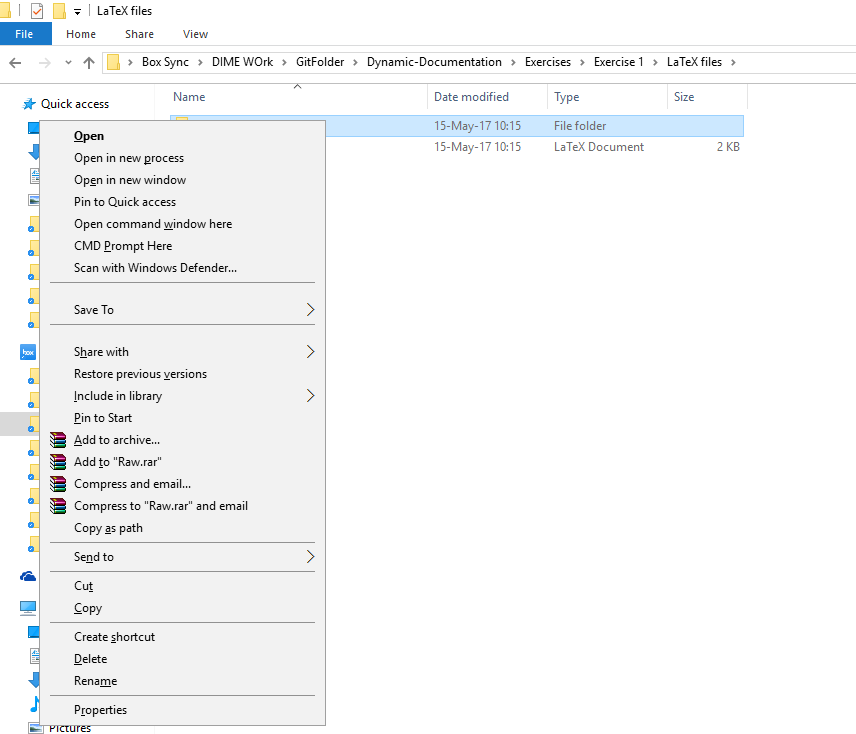
\includegraphics[width=0.7\linewidth]{img/pathwin3}
	\caption{Finding path on a Windows Computer - Solution 1}
	\label{fig:pathwin3}
\end{figure}

\subsubsection*{Option 2 - Copy as path}

\begin{figure}[H]
	\centering
	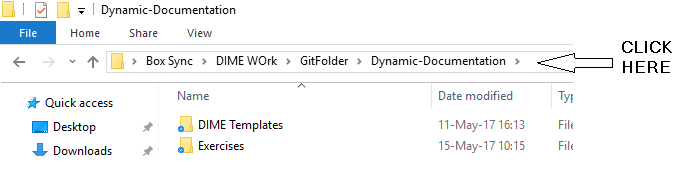
\includegraphics[width=1\linewidth]{img/pathwin}
	\caption{Finding Path on a Windows Computer}
	\label{fig:pathwin}
\end{figure}

Clicking on the bar at the top of the \texttt{File Explorer} windows where our files are saved shows us the complete path to the files in a Windows computer. \\

\begin{figure}[H]
	\centering
	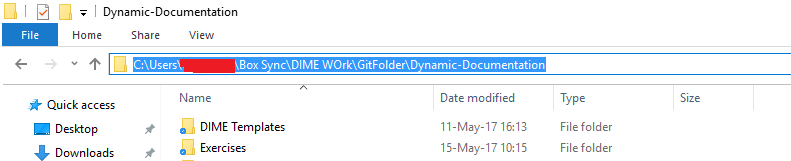
\includegraphics[width=1\linewidth]{img/pathwin2}
	\caption{Path shown on a Windows Computer}
	\label{fig:pathwin2}
\end{figure}

Once we click on the bar, the complete path to the folder is displayed, as shown in Figure \ref{fig:pathwin2}. We can then paste this path when setting the path in our Stata do-file and changing the path where it says \begin{verbatim}
global main_folder ``<<<ENTER YOUR FOLDER PATH HERE>>>''
\end{verbatim} 

\newpage

\subsection*{Annex 2 - Finding Path on a Mac}\label{annex:mac}

To copy the path on a Mac, please follow the following steps: 

\begin{itemize}
	\item Right click(or Control-click or two finger click) on the file or folder you want to copy the path of.
	\item While the right click menu appears, press the \texttt{Options} key to reveal \texttt{``Copy file as pathname''} button. This is shown in figure \ref{fig:filepathmac}.
	\item Click on that button and paste anywhere to paste the path name.
\end{itemize}
\begin{figure}[H]
	\centering
	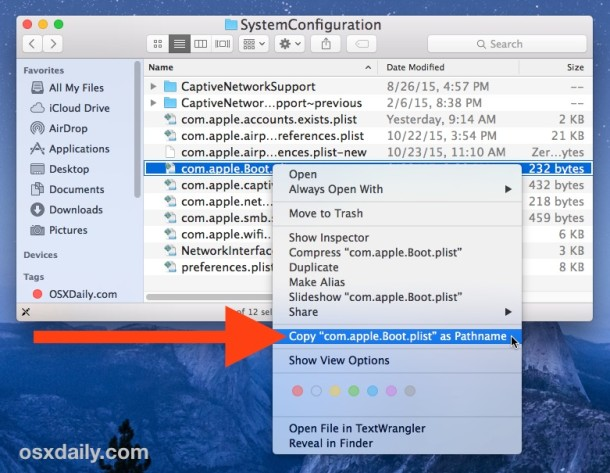
\includegraphics[width=0.7\linewidth]{../img/filepathmac}
	\caption{Finding a file path on a mac. Photo courtesy osxdaily.com}
	\label{fig:filepathmac}
\end{figure}

If you're using an older MAC computer and the option to ``Copy file as pathname'' does not show up, please follow  the following steps:

\begin{itemize}
	\item Right click(or control-click or two finger click) on your file or folder you want to copy the path of.
	\item Click on \texttt{Get Info} option that appears in the drop down menu.
	\item In the \texttt{Info} window, copy the part that appears after \textbf{Where:} and before \textbf{Created:}.
	\item Paste that part anywhere to paste the path name. 
\end{itemize}


\end{document}
